% THIS IS SIGPROC-SP.TEX - VERSION 3.1
% WORKS WITH V3.2SP OF ACM_PROC_ARTICLE-SP.CLS
% APRIL 2009
%
% It is an example file showing how to use the 'acm_proc_article-sp.cls' V3.2SP
% LaTeX2e document class file for Conference Proceedings submissions.
% ----------------------------------------------------------------------------------------------------------------
% This .tex file (and associated .cls V3.2SP) *DOES NOT* produce:
%       1) The Permission Statement
%       2) The Conference (location) Info information
%       3) The Copyright Line with ACM data
%       4) Page numbering
% ---------------------------------------------------------------------------------------------------------------
% It is an example which *does* use the .bib file (from which the .bbl file
% is produced).
% REMEMBER HOWEVER: After having produced the .bbl file,
% and prior to final submission,
% you need to 'insert'  your .bbl file into your source .tex file so as to provide
% ONE 'self-contained' source file.
%
% Questions regarding SIGS should be sent to
% Adrienne Griscti ---> griscti@acm.org
%
% Questions/suggestions regarding the guidelines, .tex and .cls files, etc. to
% Gerald Murray ---> murray@hq.acm.org
%
% For tracking purposes - this is V3.1SP - APRIL 2009

\documentclass{acm_proc_article-sp}

\usepackage{caption}
\usepackage{soul}
\usepackage{color}
\usepackage{url}
\usepackage{hyperref}
\usepackage{subfig}
\usepackage{graphicx}
%\usepackage{algpseudocode}

\begin{document}
\title{False Discovery Rate}
\subtitle{Assignment 8}
%
% You need the command \numberofauthors to handle the 'placement
% and alignment' of the authors beneath the title.
%
% For aesthetic reasons, we recommend 'three authors at a time'
% i.e. three 'name/affiliation blocks' be placed beneath the title.
%
% NOTE: You are NOT restricted in how many 'rows' of
% "name/affiliations" may appear. We just ask that you restrict
% the number of 'columns' to three.
%
% Because of the available 'opening page real-estate'
% we ask you to refrain from putting more than six authors
% (two rows with three columns) beneath the article title.
% More than six makes the first-page appear very cluttered indeed.
%
% Use the \alignauthor commands to handle the names
% and affiliations for an 'aesthetic maximum' of six authors.
% Add names, affiliations, addresses for
% the seventh etc. author(s) as the argument for the
% \additionalauthors command.
% These 'additional authors' will be output/set for you
% without further effort on your part as the last section in
% the body of your article BEFORE References or any Appendices.

%\numberofauthors{3} %  in this sample file, there are a *total*
% of EIGHT authors. SIX appear on the 'first-page' (for formatting
% reasons) and the remaining two appear in the \additionalauthors section.
%
\numberofauthors{1}
\author{
	\alignauthor Caitlin Ross\\
	\affaddr{Computer Science Department, Rensselaer Polytechnic Institute} \\
	\email{rossc3@rpi.edu}
}
% There's nothing stopping you putting the seventh, eighth, etc.
% author on the opening page (as the 'third row') but we ask,
% for aesthetic reasons that you place these 'additional authors'
% in the \additional authors block, viz.

\date{30 July 1999}
% Just remember to make sure that the TOTAL number of authors
% is the number that will appear on the first page PLUS the
% number that will appear in the \additionalauthors section.

\maketitle

\begin{abstract}
Given a file with 550 data points, I wrote a MATLAB program that calculates p-values and uses the Benjamini and Hochberg method to determine a cutoff point for the p-values to reduce the number of false positives found.  70 data points in the dataset have a p-value less than 0.05, but only 29 data points fall under the FDR cutoff using the Benjamini and Hochberg method.  We describe the program written to find these results, and display histograms and QQ plots of the data and p-values.
\end{abstract}


\section{Problem Statement}
The problem here is to take a data set, determine p-values of the data and use the Benjamini and Hochberg method to find a cutoff point for the p-values to reduce the number of false positives found.  

\section{Methods and Results}
The MATLAB program written for this assignment first reads in the data.txt file provided.  It plots a histogram of the data using 20 bins, shown in Figure 1, as well as a QQ plot, shown in Figure 2.  The homework description states that the data comes from two different normal distributions, where one is the standard normal distribution and the other has a different mean and variance.  Figure 1 appears to look similar to a standard normal distribution except that the data is skewed to the right.  The QQ plot compares the two distributions in the data by plotting their quantiles against each other.  Figure 2 shows that a lot of the points in the middle lie on a straight line.  The ends, particularly the right end, deviates from the line, probably because the data is made of a mixture of two different normal distributions.

The program then sorts the data values.  Using the standard normal distribution, it calculates the p-values of each data point by 2*cdf(-abs(data)), where cdf is the cumulative distribution function and abs is the absolute value function.  The program then plots a histogram of the p-values, again using 20 bins.  This histogram is shown in Figure 3.  P-values that are under 0.05 have the highest frequency, with the rest of the bins hovering between frequencies of 20-30 occurrences.  There are 70 data points that fall under 0.05, but some of these are likely to be false positives.    

Now the program calculates the False Discovery Rate using the Benjamini and Hochberg method, to determine the significance cutoff for p-values that should be used for this data.  We set the FDR value to 0.05 and rank the p-values $p_i$ such that $p_1 < p_2 < ... < p_n$, where n is the number of data points.  Then we find $r$ such that $p_r < \frac{r}{n}*FDR$.  Finally the program determines which data points fall under the FDR cutoff, which data points have a p-value below 0.05.  The cutoff to be used based on this method is a p-value of 0.002449.  There are 29 data points with p-values less than or equal to this cutoff, although it's expected that approximately 5\% of these values are false positives as well.    

Finally, all data points are plotted with respect to their p-values, shown in Figure 4.  Data points that fall under the FDR cutoff are plotted as a blue circle, data points that have a p-value below 0.05 but do not fall under the FDR cutoff are plotted with a red 'x', and all other data points are plotted as a green '+'.  The values that are below the FDR cutoff (blue circle) appear only on the right side of the curve, which makes sense because the histogram in Figure 1 is right-skewed.  These are probably the values from the other normal distribution used in generating the data (i.e. the one that has a different mean and variance from the standard normal distribution).  The points shown with a red 'x' are most likely data generated from the null model.  This shows why all p-values under 0.05 should not be considered significant, because given enough data points, you can get plenty of p-values that fall below 0.05 by chance.  

\begin{figure}[t]
\centering
   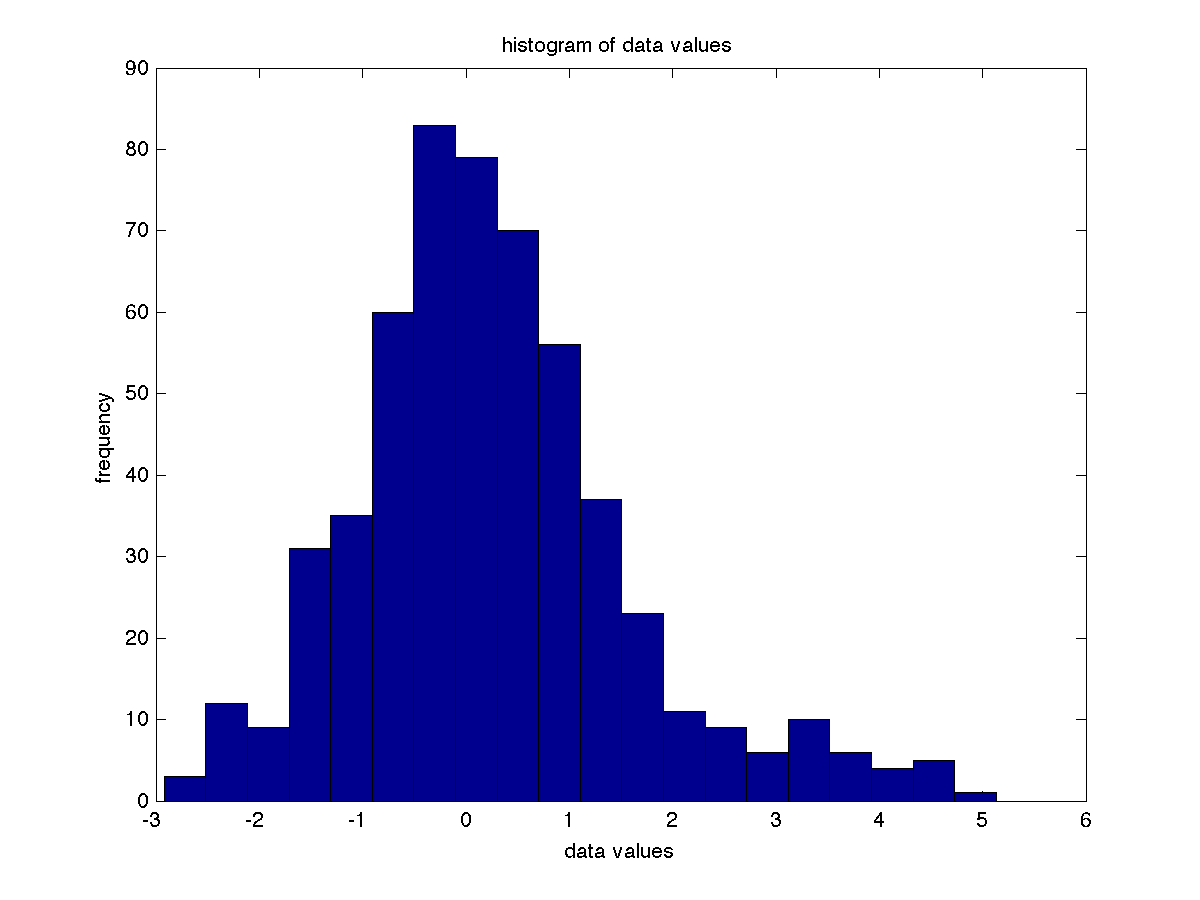
\includegraphics[width=3.5in]{hist.png}
\caption{Histogram of the given data values distributed over 20 bins}

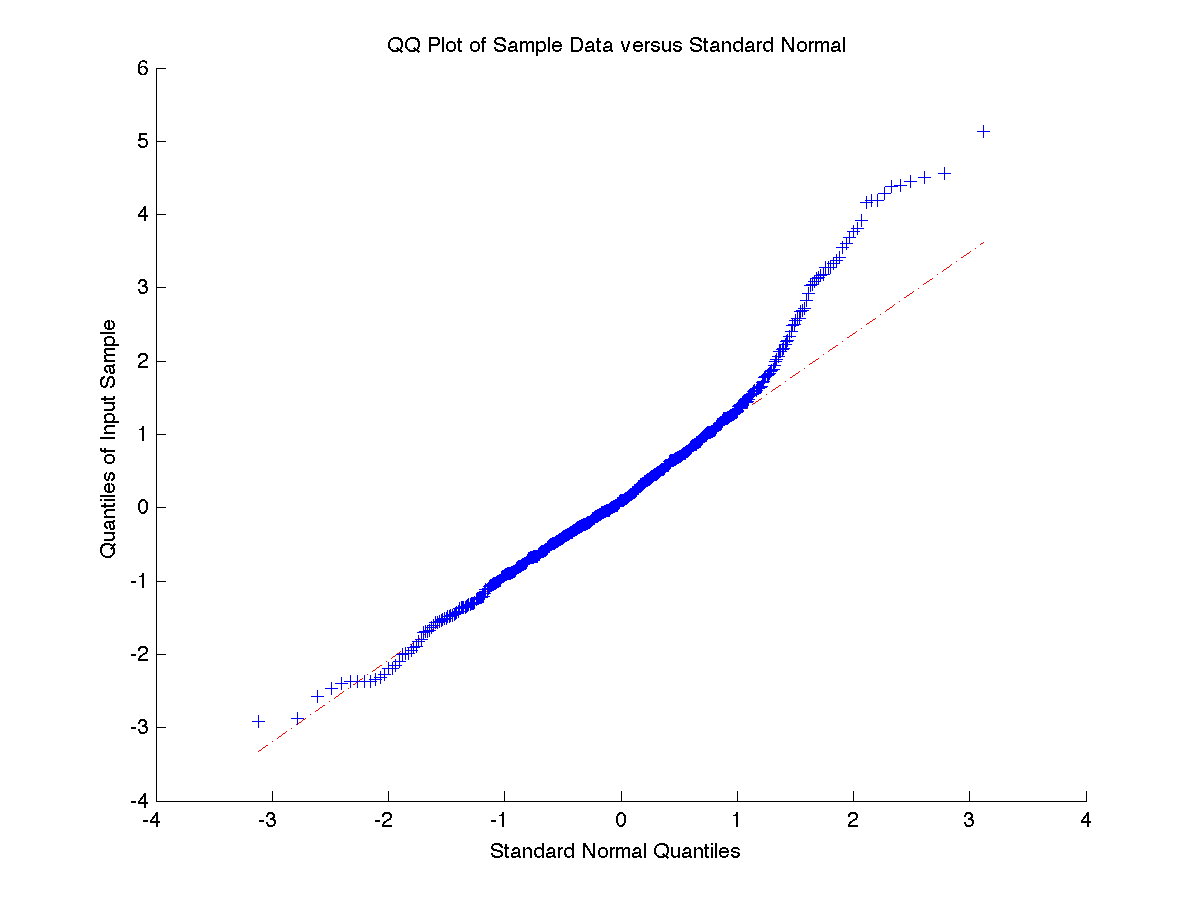
\includegraphics[width=3.5in]{qq.png}
\caption{QQ plot of the Data versus a Standard Normal Distribution}
\end{figure}

\begin{figure}[t]
\centering
   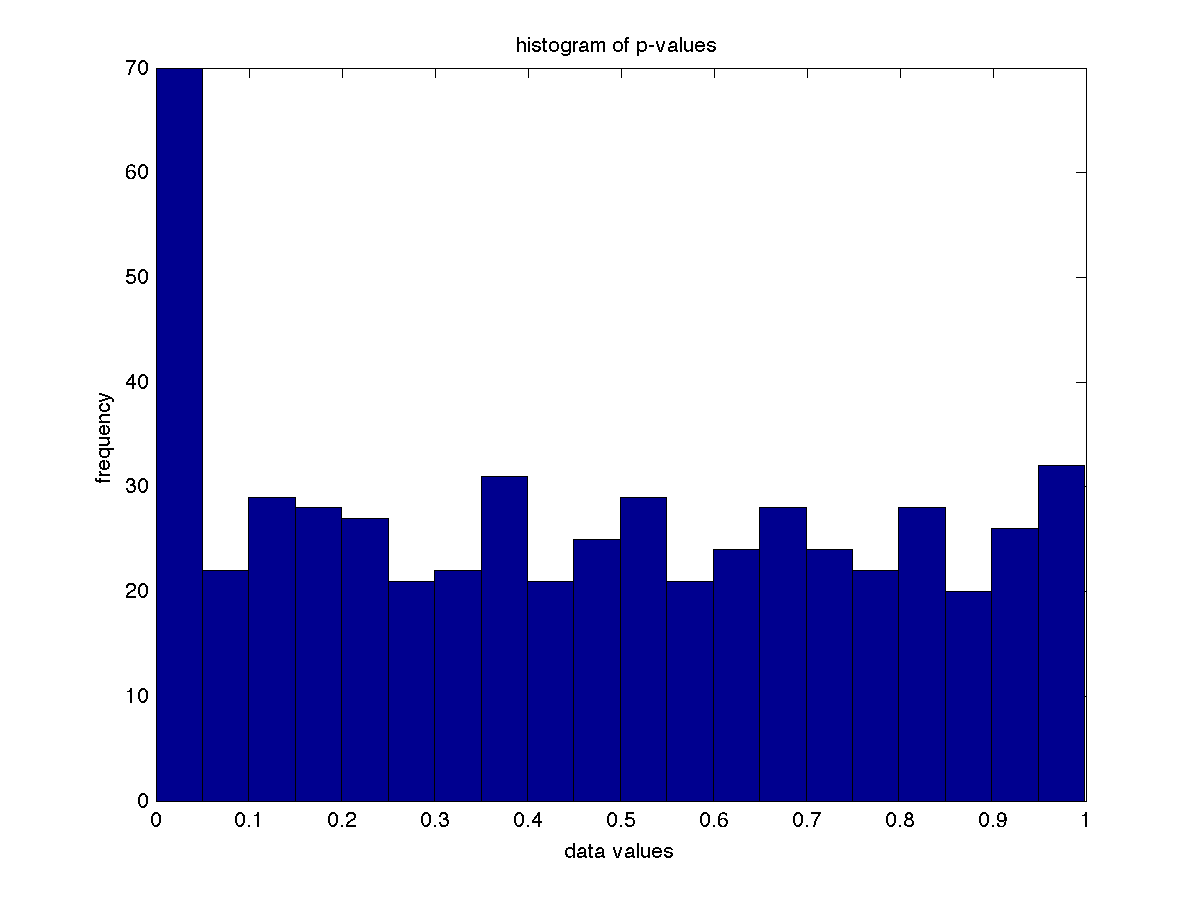
\includegraphics[width=3.5in]{hist-p.png}
\caption{Histogram of the p-values of the data distributed over 20 bins}

   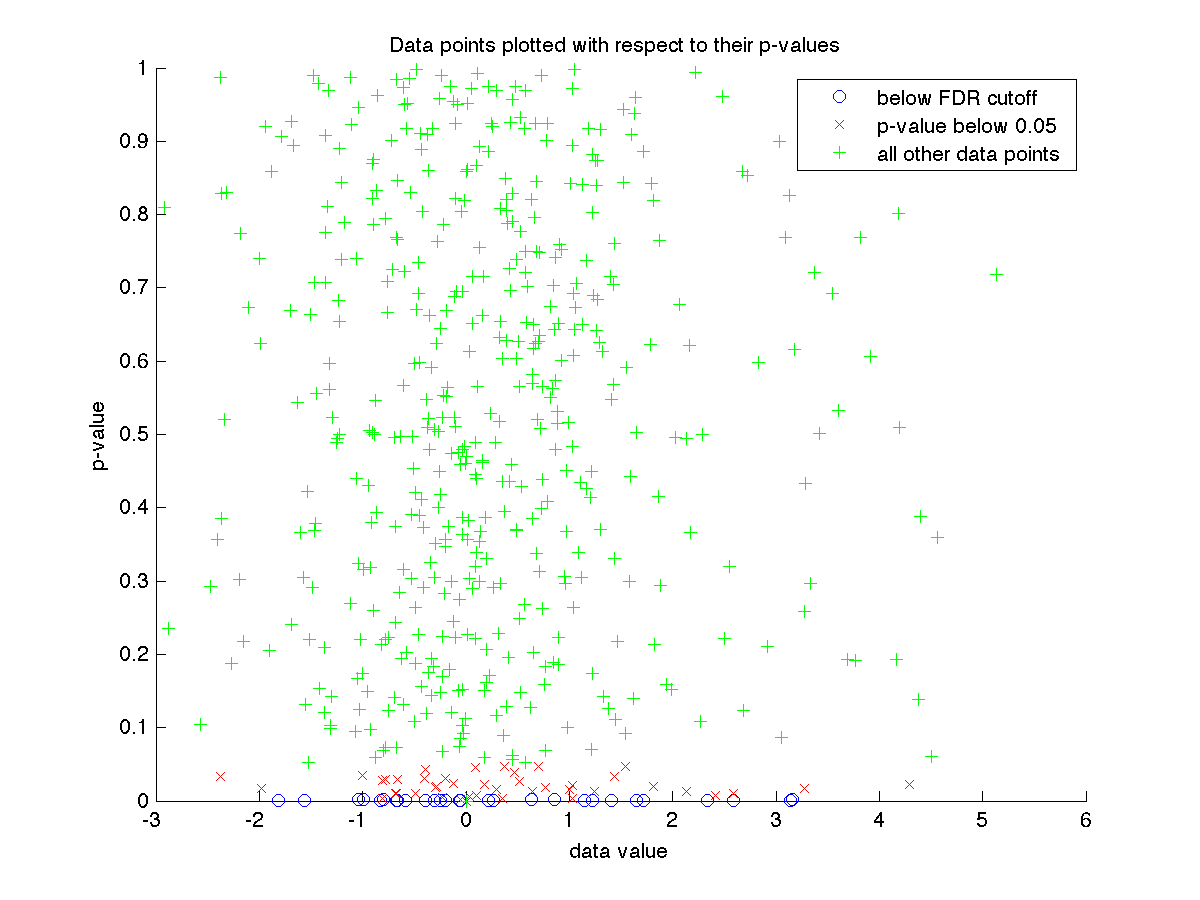
\includegraphics[width=3.5in]{all-data.png}
\caption{All data points plotted with respect to their p-values}
\end{figure}

  
%
% The following two commands are all you need in the
% initial runs of your .tex file to
% produce the bibliography for the citations in your paper.
\bibliographystyle{abbrv}
%\bibliography{sigproc}  % sigproc.bib is the name of the Bibliography in this case

% You must have a proper ".bib" file
%  and remember to run:
% latex bibtex latex latex
% to resolve all references
%
% ACM needs 'a single self-contained file'!
%
%APPENDICES are optional
%\balancecolumns

\balancecolumns
% That's all folks!
\end{document}
